% Figure 1 of the SemantEq paper ("Chains witnessing P ≃ Q"), re-laid out
% vertically for the website so that it is narrower. Same nodes, arrows,
% labels, formulas and colours as paper/section3_v3.tex; only the geometry
% changed (forward chain runs top to bottom, return chain runs up the left).
\documentclass{article}
\usepackage{tikz}
\usepackage[paperwidth=200mm,paperheight=200mm,margin=10mm]{geometry}
\pagestyle{empty}
\IfFileExists{helvet.sty}{\usepackage{helvet}}{}
\usepackage{amsmath,amssymb}
\usetikzlibrary{arrows.meta,positioning}
% palette from paper/figstyle.tex
\definecolor{seBlue}{HTML}{2A78D6}   \definecolor{seBlueBg}{HTML}{E7F0FB}
\definecolor{seGreen}{HTML}{1BAF7A}  \definecolor{seGreenBg}{HTML}{E3F5EC}
\definecolor{seYellow}{HTML}{EDA100} \definecolor{seYellowBg}{HTML}{FFF4D8}
\definecolor{seViolet}{HTML}{4A3AA7} \definecolor{seVioletBg}{HTML}{ECE9F7}
\definecolor{seGray}{HTML}{6B7280}   \definecolor{seGrayBg}{HTML}{F1F2F4}
\definecolor{seInk}{HTML}{2C3E50}    \definecolor{seInkLight}{HTML}{6B7280}
\definecolor{seArrow}{HTML}{4B5563}
\begin{document}\noindent
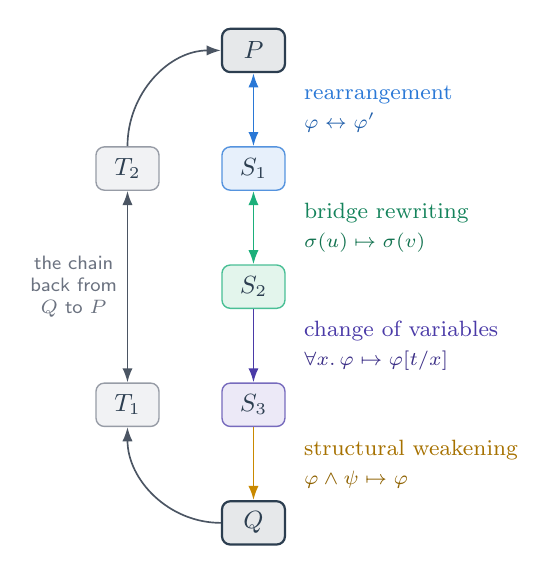
\begin{tikzpicture}[x=1mm, y=1mm, font=\sffamily,
  st/.style={draw=seGray!70, fill=seGrayBg, rounded corners=3pt, line width=0.5pt,
             minimum width=8mm, minimum height=5.5mm, inner sep=2pt, font=\small, text=seInk},
  endpt/.style={st, draw=seInk, fill=seInk!12, text=seInk, line width=0.8pt, font=\small\bfseries},
  after rearr/.style={st, draw=seBlue!80, fill=seBlueBg},
  after bridge/.style={st, draw=seGreen!80, fill=seGreenBg},
  after chvar/.style={st, draw=seViolet!75, fill=seVioletBg},
  rev/.style={{Latex[length=1.8mm,width=1.3mm]}-{Latex[length=1.8mm,width=1.3mm]}, line width=0.7pt},
  one/.style={-{Latex[length=1.8mm,width=1.3mm]}, line width=0.7pt},
  back/.style={line width=0.6pt, seArrow},
  % action name + its formula, set to the right of each arrow
  lab/.style={font=\footnotesize, inner sep=1pt, anchor=west, align=left},
  ]
% forward chain, top to bottom: one hue per action; each intermediate statement
% takes the hue of the step that produced it; the given statements are framed
\node[endpt]        (P)  at (0,0)   {$P$};
\node[after rearr]  (S1) at (0,-15) {$S_1$};
\node[after bridge] (S2) at (0,-30) {$S_2$};
\node[after chvar]  (S3) at (0,-45) {$S_3$};
\node[endpt]        (Q)  at (0,-60) {$Q$};
\draw[rev, seBlue]   (P)  -- (S1);
\draw[rev, seGreen]  (S1) -- (S2);
\draw[one, seViolet] (S2) -- (S3);
\draw[one, seYellow!85!black] (S3) -- (Q);
\node[lab, text=seBlue]              at (6,-7.5)  {rearrangement\\[1pt] {\scriptsize\color{seBlue!80!black} $\varphi\leftrightarrow\varphi'$}};
\node[lab, text=seGreen!75!black]    at (6,-22.5) {bridge rewriting\\[1pt] {\scriptsize\color{seGreen!65!black} $\sigma(u)\mapsto\sigma(v)$}};
\node[lab, text=seViolet]            at (6,-37.5) {change of variables\\[1pt] {\scriptsize\color{seViolet!80!black} $\forall x.\,\varphi\mapsto\varphi[t/x]$}};
\node[lab, text=seYellow!70!black]   at (6,-52.5) {structural weakening\\[1pt] {\scriptsize\color{seYellow!60!black} $\varphi\wedge\psi\mapsto\varphi$}};
% the chain back from Q to P, running up the left side
\node[st] (T1) at (-16,-45) {$T_1$};
\node[st] (T2) at (-16,-15) {$T_2$};
\draw[one, back] (Q.west)  to[out=180,in=-90] (T1.south);
\draw[rev, back] (T1) -- node[font=\scriptsize\sffamily, text=seInkLight, inner sep=1pt, left=2.5pt, align=center]
                   {the chain\\ back from\\ $Q$ to $P$} (T2);
\draw[one, back] (T2.north) to[out=90,in=180] (P.west);
\end{tikzpicture}
\end{document}
